\documentclass{uwstat572}
\usepackage{amsmath}
\usepackage{color}
\usepackage{graphicx}

%%\setlength{\oddsidemargin}{0.25in}
%%\setlength{\textwidth}{6in}
%%\setlength{\topmargin}{0.5in}
%%\setlength{\textheight}{9in}

\renewcommand{\baselinestretch}{1.5} 


\bibliographystyle{plainnat}

\usepackage{color}
\usepackage{ulem}
\newcommand{\vmdel}[1]{\sout{#1}}
\newcommand{\vmadd}[1]{\textbf{\color{red}{#1}}}
\newcommand{\vmcomment}[1]{({\color{blue}{VM's comment:}} \textbf{\color{blue}{#1}})}

\begin{document}
%%\maketitle

\begin{center}
  {\LARGE Bayesian Lasso}\\\ \\
  {Anonylise Wagner \\ 
    Department of Statistics, University of Washington Seattle, WA, 98195, USA
  }
\end{center}



\begin{abstract}
  The Bayesian Lasso, building on the interpretation of Tibshirani, places Laplace priors on linear regression coefficients to allow for Bayesian approaches to parameter and error estimation. An efficient Gibbs sampler allows for quick computation and may be exanded to other forms of penalized regression.
\end{abstract}

\section{Introduction}
\vmcomment{Your introduction looks more like beginning of the Methods section to me. Ideally, intro should introduce the problem without formulae. Need to motivate sparsity and give a literature review of sparse regression, explaining why it is useful and what people have done before Park and Casella paper.}
Linear regression is a broad problem with a myriad of proposed techniques for solving. At its heart, linear regression assumes that we have some vector of responses, $\boldsymbol{y}$, which depend linearly on some covariates, $\boldsymbol{X}$. Formally, accounting for an error term, we wish to fit the model \[
\boldsymbol{y} = \mu \boldsymbol{1}_n + \boldsymbol{X}\boldsymbol{\beta}+\boldsymbol{\epsilon}
\] where $\boldsymbol{y}$ is an $n \times 1$ vector, $\mu$ is the mean of $\boldsymbol{y}$, $\boldsymbol{X}$ is a matrix of regressors (typically standardized), and $\boldsymbol{\epsilon}$ is a vector of indepedent and identically distributed zero mean normal variables with an unknown variance. For the sake of this discussion we will assume that the $\boldsymbol{y}$ has zero mean ($\mu=0$), noting that in practice this can be easily achieved by subtracting the sample mean estimate.

What is really of interest is the regression coefficients, $\boldsymbol{\beta}$. These can be used for prediction when new values of regressors are given, or they may be of interest for their interpretation on the effects of certain regressor values on the dependent $\boldsymbol{y}$. Irrespective of the use, there are a number of approaches to finding the regressor coefficients. One familiar method, ordinary least squares, seeks to minimize least squares error\[
\min_{\boldsymbol{\beta}} \hspace{.1cm} (\boldsymbol{y}-\boldsymbol{X}\boldsymbol{\beta})^T(\boldsymbol{y}-\boldsymbol{X}\boldsymbol{\beta}).
\] While OLS estimates are a straight-forward and simple approach, Section~\ref{Motivation} details some of the shortcomings of this method.

Penalized regression takes a similar approach, trying to minimize the square error of predicted values, but with further constraints on regression cofficients. Of particular interest is least absolute shrinkage and selection operator (Or Lasso), which penalizes the sum of the absolute value of the coefficients. For some penalty weight $\lambda \geq 0$, the Lasso has the form \[
\min_{\boldsymbol{\beta}}  \hspace{.1cm} (\boldsymbol{y}-\boldsymbol{X}\boldsymbol{\beta})^T(\boldsymbol{y}-\boldsymbol{X}\boldsymbol{\beta})+\lambda\sum_{j=1}^p|\beta_j|.
\] In the Lasso original derivation it was noted that these estimates can be equivalently viewed as posterior modes of OLS estimates, when independent Laplace priors are placed on the $\boldsymbol{\beta}$s.\cite{tibshirani1996regression}

This idea can be expanded to other penalized regressions of the form  \[
\min_{\boldsymbol{\beta}}  \hspace{.1cm} (\boldsymbol{y}-\boldsymbol{X}\boldsymbol{\beta})^T(\boldsymbol{y}-\boldsymbol{X}\boldsymbol{\beta})+\lambda\sum_{j=1}^p|\beta_j|^q
\] for some $q\geq0$.\cite{park2008bayesian} These are collectively known as Bridge Regression, though $q=1$ (Lasso Regression) and $q=2$ (Ridge Regression) have appealing and better understood properties.

\section{Background and Motivation}\label{Motivation}
Ordinary least squares estimates are well understood, allowing for estimation of fit parameters and error suitable to many applications.\emph{\color{red} (I want to find something to cite for this) \color{black}} This method is not without its setbacks, and alternative approaches are required in many situations. 

Correlated regressor variables, for example, cause problems in estimating the statistical properties of OLS $\boldsymbol{\beta}$ estimates. OLS will also tend to fit all $\beta_j$ with at least non-zero value, as this will usually produce minor decreases in the squared error.\cite{seeger2008bayesian} This last problem helps to illustrate the desire for sparsity, a property that can be assumed \emph{a priori} or may be required due to underdetermined-ness of data.

While the Lasso does improve on OLS point estimates, until recently error estimates were difficult to derive. The more desirous property of the Lasso is its ability to produce sparce estimates of parameters. It accomplishes this task by restricting solutions onto an $L_1$ 'ball' around the origin. This is more obvious from the dual formulation, 
\begin{align*}
\min_{\boldsymbol{\beta}}  \hspace{.1cm} &(\boldsymbol{y}-\boldsymbol{X}\boldsymbol{\beta})^T(\boldsymbol{y}-\boldsymbol{X}\boldsymbol{\beta})\\
\text{subject to} \hspace{.1cm}&\sum_{j=1}^p|\beta_j|\leq r
\end{align*}
for some $r$ determined by $\lambda$. Figure~\ref{LassoPlot} shows how this penalization compares to a Ridge Regression, Bridge Regression with $q=2$ which restricts solutions onto an $L_2$ ball.\cite{park2008bayesian}

\begin{figure}\label{LassoPlot}
  \centering
    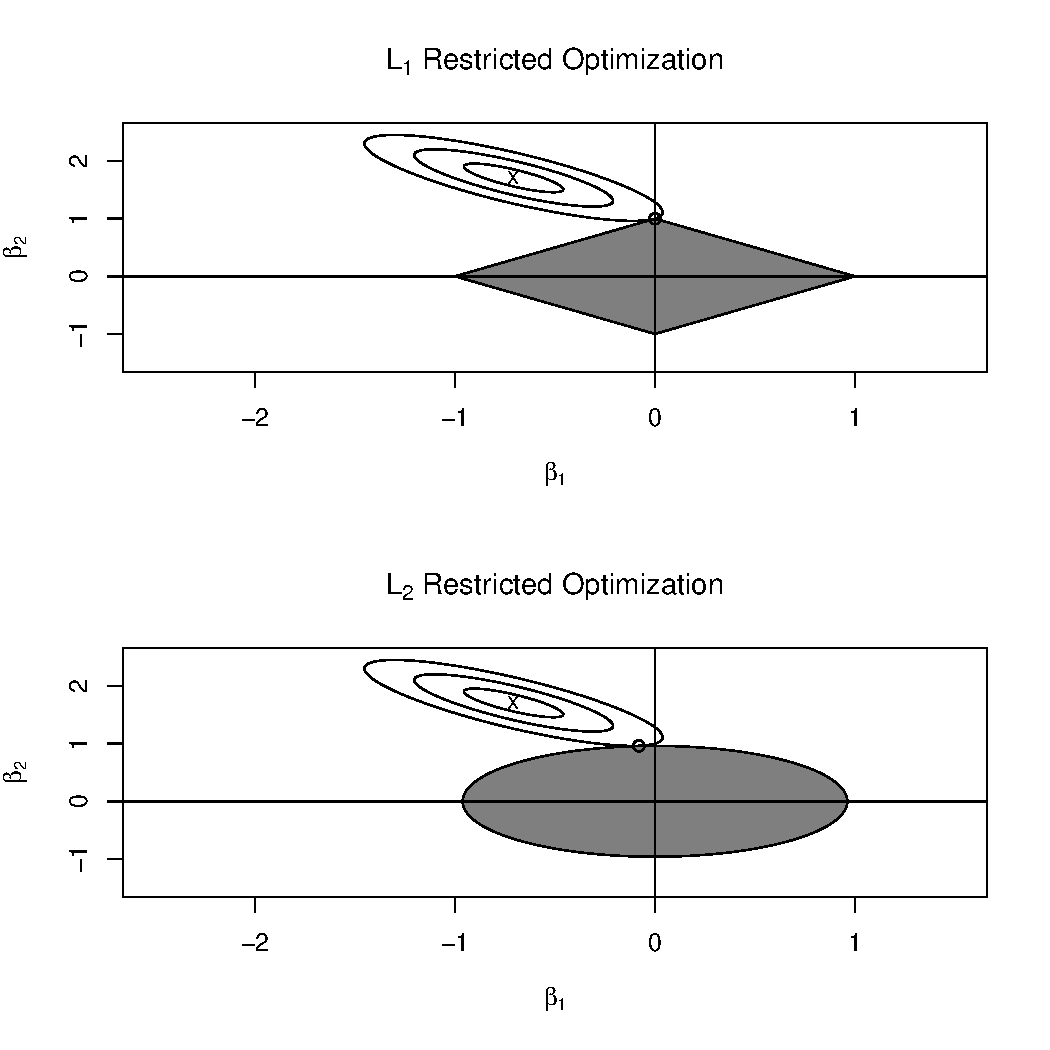
\includegraphics[width=0.7\textwidth]{LassoPlot.pdf}
  \caption{This example illustrates the tendancy for Lasso estimates to be driven to 0, compared with Ridge Regression estimates which are close to but not exactly 0 for $\beta_1$. \emph{\color{red} (I want to make this side by side, and 1:1)\color{black}}}
\end{figure}

While sparcity may be an \emph{a priori} assumption made about the data, underdetermined data requires this assumption to create useful models. One common field often presented with this problem is the study of gene expression, where there may be thousands to hundreds of thousands of predictors but only a few hundred data points.\cite{seeger2008bayesian}

The Bayesian Lasso, in keeping with Tibshirani's original interpretation, places independent Laplace (or double exponential) distributions on the parameters. Specifically, \[
\pi(\beta|\sigma^2)=\prod_{j=1}^p\frac{\lambda}{2\sqrt{\sigma^2}}e^{-\lambda |\beta_j|/\sqrt{\sigma^2}}
\] is placed on each distribution, which results in a unimodal posterior. Other prior distributions have been considred, but unimodality is key for Lasso estimates as non-unimodal posterior distributions cause convergence problems.

In the paper by Park and Casella, they produce a heirarchical models along with a Gibbs sampling technique to sample from posterior distributions. Alongside this formulation they also present an approach to a data-driven estimation for $\lambda$ hyperparameters.\cite{park2008bayesian}
=======
\section{Background and Motivation}
\vmcomment{I don't think you need a separate Background section; make it a Methods subsection if needed}

\section{Methods}

\section{Results}

\section{Discussion}

\bibliography{stat572}

\end{document}









